% Options for packages loaded elsewhere
\PassOptionsToPackage{unicode}{hyperref}
\PassOptionsToPackage{hyphens}{url}
%
\documentclass[
  ignorenonframetext,
  aspectratio=169,
]{beamer}
\usepackage{pgfpages}
%\usepackage{arxiv}
%\usepackage[utf8]{inputenc} % allow utf-8 input
%\usepackage[T1]{fontenc}    % use 8-bit T1 fonts
%\usepackage{hyperref}       % hyperlinks
%\usepackage{url}            % simple URL typesetting
%\usepackage{nicefrac}       % compact symbols for 1/2, etc.
%\usepackage{microtype}      % microtypography
%\usepackage{graphicx}
%\usepackage[square, sort, numbers]{natbib}
%\usepackage{doi}
% \usepackage{subfig}
% \usepackage{cleveref}
\usepackage{booktabs}       % professional-quality tables
\usepackage{amsfonts}       % blackboard math symbols
\usepackage{amsmath}
\usepackage{multicol}
\usepackage{subcaption}
\usepackage{pgfplots}
\pgfplotsset{compat=1.9}

\usepackage{tikz}
\usetikzlibrary{positioning, fit, arrows, shapes}
\tikzset{>=latex}
\usepackage{ifthen}
\usepackage{intcalc}
%\graphicspath{{./gfx/}}
\usepackage{fontspec}

\newcommand{\empt}[2]{$#1^{\langle #2 \rangle}$}

% \usepgfplotslibrary{external}
% \tikzexternalize

\setmainfont[UprightFont={* Light},
    BoldFont={*  Medium},
    ItalicFont={* Light Italic},
    BoldItalicFont={* Medium Italic},
]{Noto Serif}


\makeatletter
\long\def\ifnodedefined#1#2#3{%
    \@ifundefined{pgf@sh@ns@#1}{#3}{#2}%
}
\makeatother
\setbeamertemplate{caption}[numbered]
\setbeamertemplate{caption label separator}{: }
\setbeamercolor{caption name}{fg=normal text.fg}
\beamertemplatenavigationsymbolsempty
% Prevent slide breaks in the middle of a paragraph
\widowpenalties 1 10000
\raggedbottom
\setbeamertemplate{part page}{
  \centering
  \begin{beamercolorbox}[sep=16pt,center]{part title}
    \usebeamerfont{part title}\insertpart\par
  \end{beamercolorbox}
}
\setbeamertemplate{section page}{
  \centering
  \begin{beamercolorbox}[sep=12pt,center]{part title}
    \usebeamerfont{section title}\insertsection\par
  \end{beamercolorbox}
}
\setbeamertemplate{subsection page}{
  \centering
  \begin{beamercolorbox}[sep=8pt,center]{part title}
    \usebeamerfont{subsection title}\insertsubsection\par
  \end{beamercolorbox}
}
\AtBeginPart{
  \frame{\partpage}
}
\AtBeginSection{
  \ifbibliography
  \else
    \frame{\sectionpage}
  \fi
}
\AtBeginSubsection{
  \frame{\subsectionpage}
}
\usepackage{lmodern}
\usepackage{amssymb,amsmath}
\usepackage{ifxetex,ifluatex}
\ifnum 0\ifxetex 1\fi\ifluatex 1\fi=0 % if pdftex
  \usepackage[T1]{fontenc}
  \usepackage[utf8]{inputenc}
  \usepackage{textcomp} % provide euro and other symbols
\else % if luatex or xetex
  \usepackage{unicode-math}
  \defaultfontfeatures{Scale=MatchLowercase}
  \defaultfontfeatures[\rmfamily]{Ligatures=TeX,Scale=1}
\fi
\usetheme[]{Metropolis}
% Use upquote if available, for straight quotes in verbatim environments
\IfFileExists{upquote.sty}{\usepackage{upquote}}{}
\IfFileExists{microtype.sty}{% use microtype if available
  \usepackage[]{microtype}
  \UseMicrotypeSet[protrusion]{basicmath} % disable protrusion for tt fonts
}{}
\makeatletter
\@ifundefined{KOMAClassName}{% if non-KOMA class
  \IfFileExists{parskip.sty}{%
    \usepackage{parskip}
  }{% else
    \setlength{\parindent}{0pt}
    \setlength{\parskip}{6pt plus 2pt minus 1pt}}
}{% if KOMA class
  \KOMAoptions{parskip=half}}
\makeatother
\usepackage{xcolor}
\IfFileExists{xurl.sty}{\usepackage{xurl}}{} % add URL line breaks if available
\IfFileExists{bookmark.sty}{\usepackage{bookmark}}{\usepackage{hyperref}}
\hypersetup{
  pdftitle={Generative Modelling of Sequential Data},
  pdfauthor={Magnus Berg Sletfjerding},
  hidelinks,
  pdfcreator={LaTeX via pandoc}}
\urlstyle{same} % disable monospaced font for URLs
\newif\ifbibliography
\usepackage{longtable,booktabs}
\usepackage{caption}
% Make caption package work with longtable
\makeatletter
\def\fnum@table{\tablename~\thetable}
\makeatother
\setlength{\emergencystretch}{3em} % prevent overfull lines
\providecommand{\tightlist}{%
  \setlength{\itemsep}{0pt}\setlength{\parskip}{0pt}}
\setcounter{secnumdepth}{-\maxdimen} % remove section numbering

\title{Generative Modelling of Sequential Data}
\subtitle{M.Sc. thesis in collaboration with Corti ApS}
\author{Magnus Berg Sletfjerding}
\date{February 9th, 2022}

\begin{document}
\frame{\titlepage}

\begin{frame}{Contents}
\protect\hypertarget{contents}{}
\tableofcontents
\end{frame}

\hypertarget{introduction}{%
\section{Introduction}\label{introduction}}

\begin{frame}{Supervised and Unsupervised learning}
\protect\hypertarget{supervised-and-unsupervised-learning}{}
\begin{figure}
\centering
\resizebox{!}{0.5\textheight}{
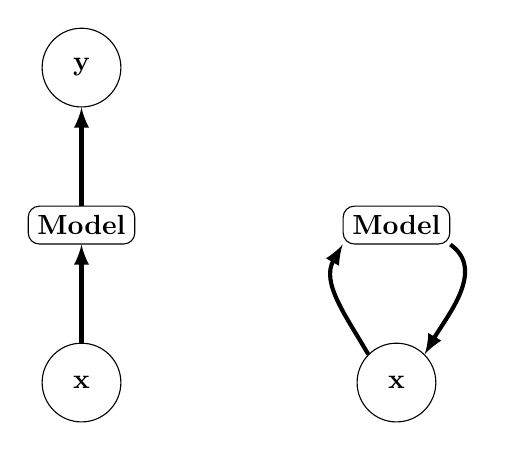
\begin{tikzpicture}


    % \foreach \x in {1,2,3,4}{
    %     \node[circle,draw,fill=white!50, minimum height=10mm,] (Input-\x) at (\intcalcMul{2}{\x},0) {$x_{\x}$};

    %     \node[rectangle, draw, rounded corners, above=of Input-\x] (Model-\x)  {Model};

    %     \node[circle,draw,fill=white!50, minimum height=10mm, above=of Model-\x] (Input-\x) {$y_{\x}$};

    % }

    \node[circle,draw,fill=white!50, minimum height=10mm,] (Input) at (0,0) {$\mathbf{x}$};

    \node[rectangle, draw, rounded corners] (Model) at (0,2)  {\textbf{Model}};

    \node[circle,draw,fill=white!50, minimum height=10mm] at (0,4) (Output) {$\mathbf{y}$};

    \draw[->, line width=1.5] (Input.north) -- (Model.south);

    \draw[->, line width=1.5] (Model.north) -- (Output.south);


    \node[circle,draw,fill=white!50, minimum height=10mm,] (Input-U) at (4,0) {$\mathbf{x}$};

    \node[rectangle, draw, rounded corners] (Model-U) at (4,2)  {\textbf{Model}};

    \draw[->, line width=1.5] (Input-U.north west)  to[out=120, in=-120] (Model-U.south west);

    \draw[->, line width=1.5] (Model-U.south east)  to[out=-35, in=60] (Input-U.north east);
    % \node[right=of Input-15, align=right] {
    % \textbf{Original Input}
    % };
    % \node[right=of Stack-4, align=right] {
    % \textbf{Stacked Input}
    % };

\end{tikzpicture}%
}\end{figure}

\begin{columns}[T]
\begin{column}{0.48\textwidth}
\begin{block}{Supervised Learning}
\protect\hypertarget{supervised-learning}{}
Learns a mapping from data \(\mathbf{x}\) to labels \(\mathbf{y}\):\\
\[
p(\mathbf{y}|\mathbf{x}) = \sum^N_{i=1} p(y_i| x_i)
\]
\end{block}
\end{column}

\begin{column}{0.48\textwidth}
\begin{block}{Unsupervised Learning}
\protect\hypertarget{unsupervised-learning}{}
Learns the structure of the data \(\mathbf{x}\): \[
p(\mathbf{x}) = \sum^N_{i=1} p(x_t)
\]
\end{block}
\end{column}
\end{columns}
\end{frame}

\begin{frame}{Why study hierarchies of information in sequences?}
\protect\hypertarget{why-study-hierarchies-of-information-in-sequences}{}
\begin{itemize}
\item
  Most data we work with has some hierarchical structure

  \begin{itemize}
  \tightlist
  \item
    Text
  \item
    Video
  \item
    Proteins/DNA
  \end{itemize}
\item
  Human brains process hierarchies of information natively

  \begin{itemize}
  \tightlist
  \item
    Human-like AI requires hierarchical processing
  \end{itemize}
\item
  All real-world data has a sequential dimension - time!
\end{itemize}
\end{frame}

\begin{frame}{Unsupervised sequence modeling}
\protect\hypertarget{unsupervised-sequence-modeling}{}
Unsupervised sequence modeling optimize the likelihood \(p(\cdot)\) of
the data \(\mathbf{x}\), calculated by conditioning the likelihood of
\(x_t\) on previous timesteps: \[
p(\mathbf{x}) = \prod^N_{t=1}  p(x_t | x_{<t}) , \hspace{1cm}  \mathbf{x}\in \mathbb{R}^N
\]
\end{frame}

\begin{frame}{Recurrent vs.~Convolutional Autoregressive models}
\protect\hypertarget{recurrent-vs.-convolutional-autoregressive-models}{}
\begin{figure}[t]  
\centering 
  \begin{subfigure}[b]{0.45\linewidth}
  \resizebox{\columnwidth}{!}
    {
    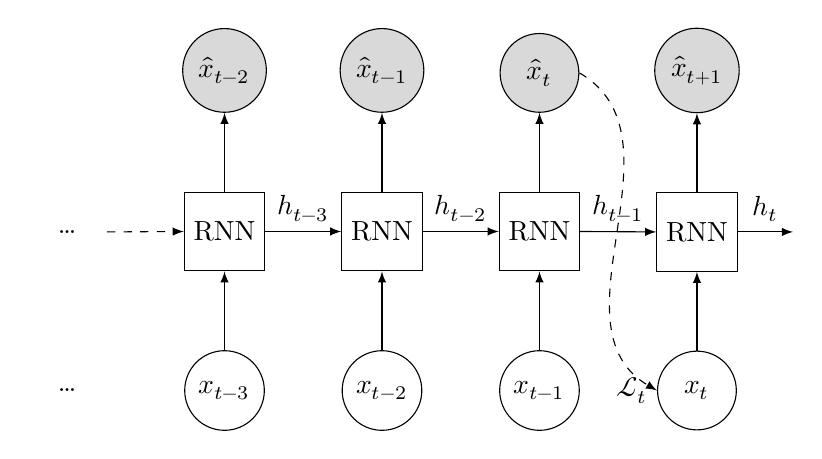
\begin{tikzpicture}%[transform canvas={scale=0.5}]
    % Input nodes
    \node[circle, 
        minimum size = 10mm,
        draw,
        % fill=orange!30
    ] (Input-0) at (0,0) {$x_{t}$};
    
    \foreach \i in {1,2,3}
    {
        \node[circle, 
            minimum size = 10mm,
            draw,
            % fill=orange!30,
            ] (Input-\i) at (-2*\i,0) {$x_{t-\i}$};
    }
    \node[circle, minimum size = 10mm,% fill=orange!30,
            ] (Input-ldots) at (-2*4,0) {\dots};
    \node[circle, minimum size = 10mm,% fill=orange!30,
            above=of Input-ldots] (RNN-ldots) {\dots};
    
    % Draw RNNs
    \foreach \i in {0,1,2,3}
    {
    \node[rectangle, draw, above=of Input-\i, minimum height=1cm, minimum width=1cm] (RNN-\i) {RNN};
    }

    % Draw Outputs

    \node[circle, minimum size = 10mm, draw, fill=gray!30, above=of RNN-0] (Output-0) {$\hat{x}_{t+1}$};
    \node[circle, minimum size = 10mm, draw, fill=gray!30, above=of RNN-1] (Output-1) {$\hat{x}_{t}$};    
    \node[circle, minimum size = 10mm, draw, fill=gray!30, above=of RNN-2] (Output-2) {$\hat{x}_{t-1}$};
    \node[circle, minimum size = 10mm, draw, fill=gray!30, above=of RNN-3] (Output-3) {$\hat{x}_{t-2}$};
    % draw arrows
    \foreach \i in {0,1,2,3}
    {
    \draw[->] (Input-\i.north) -- (RNN-\i.south);
    \draw[->] (RNN-\i.north) -- (Output-\i.south);
    }

    \draw[->,dashed] (RNN-ldots.east) -- (RNN-3.west) ;
    \draw[->] (RNN-3.east) -- (RNN-2.west) node[midway, above] {$h_{t-3}$};
    \draw[->] (RNN-2.east) -- (RNN-1.west) node[midway, above] {$h_{t-2}$};
    \draw[->] (RNN-1.east) -- (RNN-0.west) node[midway, above] {$h_{t-1}$};
    \draw[->] (RNN-0.east) -- +(20pt,0) node[midway, above] {$h_{t}$};
    
    % % Arrow from Hat to next 
    % \draw[->] (Output-3.east) edge[bend right=15] (Input-2.west);
    % \draw[->] (Output-2.east) edge[bend right=15] (Input-1.west);
    % \draw[->] (Output-1.east) edge[bend right=15] (Input-0.west);

    \draw[->, dashed] (Output-1.east) 
        to[out=-30, in=150]
        % edge[bend left=30] 
    (Input-0.west) node[left] {$\mathcal{L}_{t}$}   ;

\end{tikzpicture}%%
    }
  \end{subfigure}
  \hfill
  \begin{subfigure}[b]{0.45\linewidth}
  \resizebox{\columnwidth}{!}
    {
    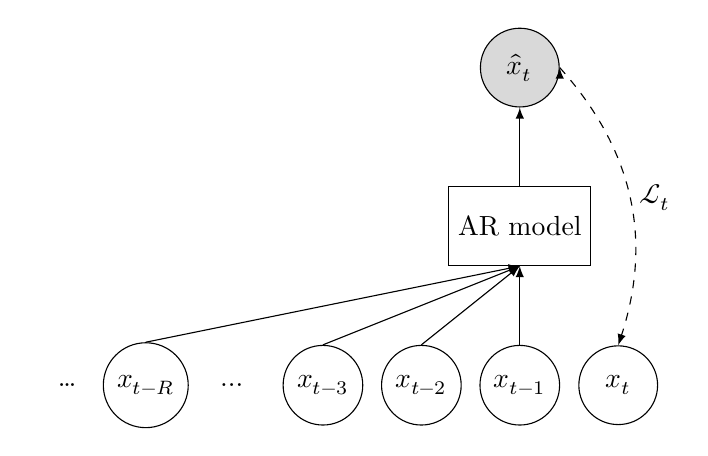
\begin{tikzpicture}
    % Input nodes
    \node[circle, 
    minimum size = 10mm,
    draw,
    % fill=orange!30
    ] (Input-0) at (0,0) {$x_{t}$};
    
    \foreach \i in {1,2,3}
    {
        \node[circle, 
            minimum size = 10mm,
            draw,
            % fill=orange!30,
            ] (Input-\i) at (-1.25*\i,0) {$x_{t-\i}$};
    }
    
    % Network
    \node[rectangle, draw, above=of Input-1, minimum height=1cm, minimum width=1cm] (AR-Model) {AR model};
    
    % dots node
    \node[circle, 
        minimum size = 10mm,
        % draw,
        % fill=orange!30,
        ] (Input-dots) at (-4.87,0) {$\dots$};
    % R node at pos 5 
    \node[circle, 
            minimum size = 10mm,
            draw,
            % fill=orange!30,
            ] (Input-R) at (-6,0) {$x_{t-R}$};
            
    \node[circle, 
        minimum size = 10mm,
        % draw,
        % fill=orange!30,
        ] (Input-R-1) at (-7,0) {\dots};
    
    % \draw[->] (Input-R.north) -- (AR-Model.south);
    
    % Arrows
    \foreach \i in {1,2,3,R}
    {
        \draw[->] (Input-\i.north) -- (AR-Model.south);
    }

    % Output
    \node[circle,
     minimum size = 10mm,
    fill=gray!30,
    draw,
    above=of AR-Model
    ] (Output-0) {$\hat{x}_{t}$};

    \draw[->] (AR-Model.north) -- (Output-0.south);

    % Arrow from Hat to next 
    \draw[->, dashed] (Output-0.east) edge[bend left=30] node[midway, right] {$\mathcal{L}_{t}$} (Input-0.north) ;

\end{tikzpicture}%%
    }
  \end{subfigure}
  %\caption{
%  Comparison between Recurrent and Autoregressive architectures for computing $\hat{x}_t$. Note that to estimate $\hat{x}_t$ accurately, the RNN needs to calculate its output multiple times, while the autoregressive model only needs to calculate its output once. 
  %}
\end{figure}  

\begin{columns}[T]
\begin{column}{0.48\textwidth}
\begin{block}{Recurrent architectures}
\protect\hypertarget{recurrent-architectures}{}
Condition \(p(x_t|x_{<t})\) through one or more hidden states \(h_t\)
passed between timesteps: \[
p(x_t, h_t | x_{<t}) = p(x_t | x_{t-1}, h_{t-1})
\]
\end{block}
\end{column}

\begin{column}{0.48\textwidth}
\begin{block}{Autoregressive Architectures}
\protect\hypertarget{autoregressive-architectures}{}
Condition \(p(x_t|x_{<t})\) by viewing a receptive field of size \(R\)
of the input sequence. \[
p(\mathbf{x}) = \prod^N_{t=R+1} p(x_t | x_{\geq t-R+1, <t})
\]
\end{block}
\end{column}
\end{columns}
\end{frame}

\begin{frame}{WaveNet - Convolutional Autoregressive Sequence Modelling}
\protect\hypertarget{wavenet---convolutional-autoregressive-sequence-modelling}{}
\begin{figure}
    \centering
    \resizebox{0.7\columnwidth}{!}{
    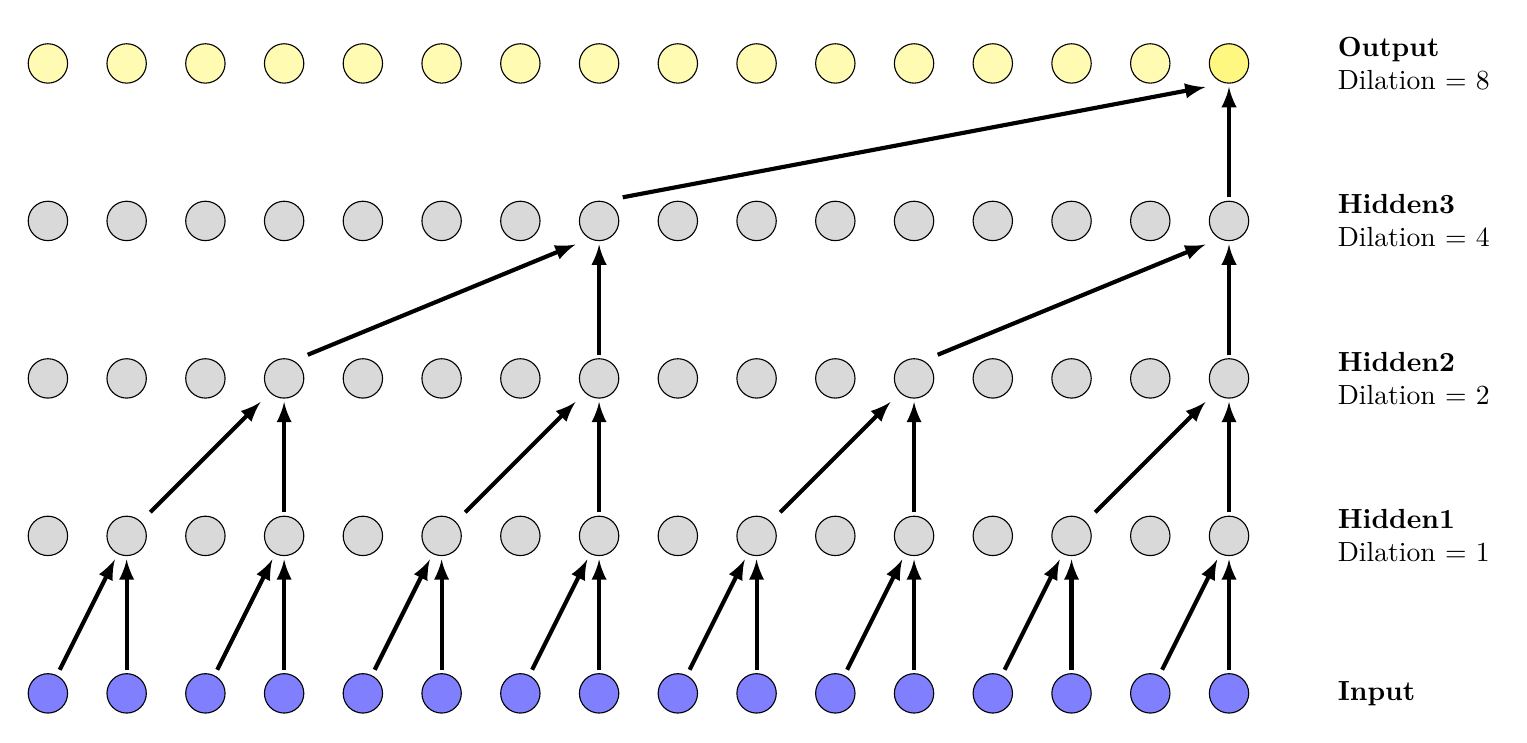
\begin{tikzpicture}
\node[circle,draw,fill=blue!50,minimum height=5mm,] (Input-15) at (15,0) {};
\node[circle,draw,fill=gray!30,minimum height=5mm] (Hidden1-15) at (15,2) {};
\node[circle,draw,fill=gray!30,minimum height=5mm] (Hidden2-15) at (15,4) {};
\node[circle,draw,fill=gray!30,minimum height=5mm] (Hidden3-15) at (15,6) {};
\node[circle,draw,fill=yellow!50,minimum height=5mm] (Output-15) at (15,8) {};

\node[right=of Input-15, align=left] {
\textbf{Input}
};
\node[right=of Hidden1-15, align=left] {
\textbf{Hidden1}\\
Dilation = 1
};
\node[right=of Hidden2-15, align=left] {
\textbf{Hidden2}\\
Dilation = 2
};
\node[right=of Hidden3-15, align=left] {
\textbf{Hidden3}\\
Dilation = 4
};
\node[right=of Output-15, align=left] {
\textbf{Output}\\
Dilation = 8
};


\draw[->, line width=1.5] (15,0.3) -- (15, 1.7);
\draw[->, line width=1.5] (15,2.3) -- (15, 3.7);
\draw[->, line width=1.5] (15,4.3) -- (15, 5.7);
\draw[->, line width=1.5] (15,6.3) -- (15, 7.7);


\foreach \x in {0, 1, ..., 14}{
	\ifthenelse{\intcalcMod{\x}{2}=0}{
		\draw[->, line width=1.5] (\x+0.15,0.3) -- (\x+0.85, 1.7);
	}{
		\draw[->, line width=1.5] (\x,0.3) -- (\x, 1.7);
	}
	\ifthenelse{\intcalcMod{\x}{4}=1}{
		\draw[->, line width=1.5] (\x+0.3,2.3) -- (\x+1.7, 3.7);
	}{}
	\ifthenelse{\intcalcMod{\x}{4}=3}{
		\draw[->, line width=1.5] (\x,2.3) -- (\x, 3.7);
	}{}
	\ifthenelse{\intcalcMod{\x}{8}=3}{
		\draw[->, line width=1.5] (\x+0.3,4.3) -- (\x+3.7, 5.7);
	}{}
	\ifthenelse{\intcalcMod{\x}{8}=7}{
		\draw[->, line width=1.5] (\x,4.3) -- (\x, 5.7);
	}{}
	\ifthenelse{\intcalcMod{\x}{16}=7}{
		\draw[->, line width=1.5] (\x+0.3,6.3) -- (\x+7.7, 7.7);
	}{}
	\ifthenelse{\intcalcMod{\x}{16}=15}{
		\draw[->, line width=1.5] (\x,6.3) -- (\x, 7.7);
	}{}
}

\foreach \x in {0, 1, ..., 14}{
	\draw[fill=blue!50] (\x,0) circle [radius=0.25];
	\draw[fill=gray!30] (\x, 2) circle [radius=0.25];
	\draw[fill=gray!30] (\x, 4) circle [radius=0.25];
	\draw[fill=gray!30] (\x, 6) circle [radius=0.25];
	\draw[fill=yellow!30] (\x, 8) circle [radius=0.25];
}


% caption on the right
% \node[right=of Input-15] {Hello};


\end{tikzpicture}%}
    %\caption{
    %Illustration of a 4-layer WaveNet architecture with exponentially increasing dilation $d_i=2^i, i\in [0, 3]$ and kernel size 2.
    %This results in a receptive field of size $2^4=16$. 
    %}
    %\label{fig:intro-wavenet}
\end{figure}

\begin{itemize}
\tightlist
\item
  Common vocoder in Speech To Text production systems
\item
  Makes use of dilated convolution to inflate receptive field
\item
  No ``hidden state'' for representing earlier timesteps
\item
  Constrained to look back within receptive field
\end{itemize}
\end{frame}

\hypertarget{problem-and-hypotheses}{%
\section{Problem and Hypotheses}\label{problem-and-hypotheses}}

\begin{frame}{Main Problem with WaveNet \ldots{}}
\protect\hypertarget{main-problem-with-wavenet}{}
\begin{itemize}
\tightlist
\item
  Local signal structure\\
\item
  Missing long-range correlations
\item
  Low receptive field (300ms)
\item
  Generated audio sounds like babbling if not conditioned on phoneme or
  text representations
\end{itemize}
\end{frame}

\begin{frame}{Hypotheses Investigated}
\protect\hypertarget{hypotheses-investigated}{}
\begin{enumerate}
\tightlist
\item
  WaveNet's receptive field is the main limiting factor for modeling
  long-range dependencies.
\item
  WaveNet's stacked convolutional layers learn good representations of
  speech.
\item
  WaveNet's hierarchical structure makes it suitable to learn priors
  over representations of speech such as text.
\item
  A large WaveNet architecture trained on speech can generate coherent
  words and sentence fragments
\end{enumerate}
\end{frame}

\hypertarget{experiments}{%
\section{Experiments}\label{experiments}}

\begin{frame}{Experiment overview}
\protect\hypertarget{experiment-overview}{}
\begin{enumerate}
\tightlist
\item
  Expanding Receptive Field by Stacking
\item
  Latent Space of Stacked WaveNets
\item
  WaveNet as a Language Model
\item
  WaveNet as an ASR preprocessor
\end{enumerate}
\end{frame}

\begin{frame}{Expanding Receptive Field by Stacking - Setup}
\protect\hypertarget{expanding-receptive-field-by-stacking---setup}{}
\begin{block}{Hypothesis tested}
\protect\hypertarget{hypothesis-tested}{}
\begin{enumerate}[<+->]
\tightlist
\item
  WaveNet's receptive field is the main limiting factor for modeling
  long-range dependencies.
\end{enumerate}
\end{block}

\begin{block}{Setup}
\protect\hypertarget{setup}{}
Transform x as:

\begin{figure}
\centering
\resizebox{\columnwidth}{!}{
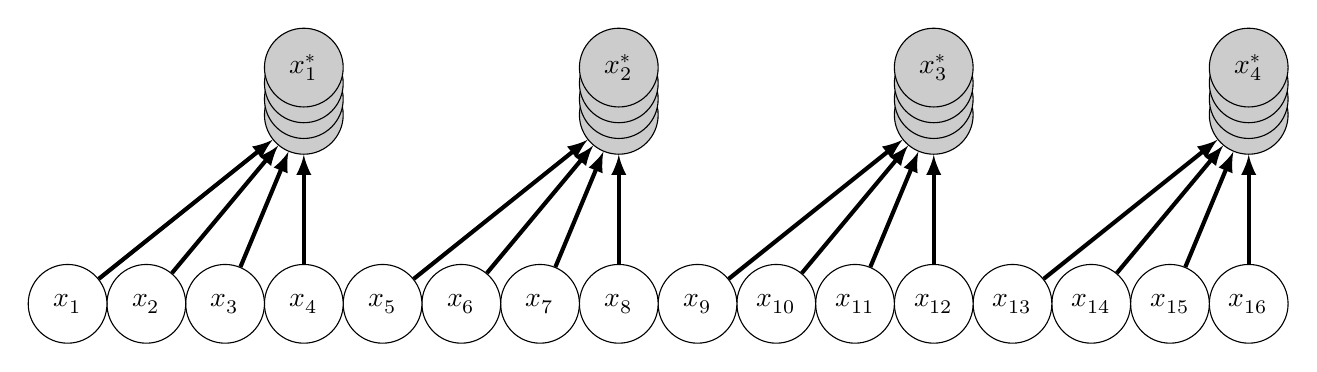
\begin{tikzpicture}
    \foreach \x in {16, 12, 8, 4} {
            \node[circle, draw, fill=black!20, minimum height=10mm,] (Stack-\intcalcDiv{\x}{4}-0) at (\x, 2.4) {};

            \node[circle, draw, fill=black!20, minimum height=10mm,] (Stack-\intcalcDiv{\x}{4}-1) at (\x, 2.6) {};

            \node[circle, draw, fill=black!20, minimum height=10mm,] (Stack-\intcalcDiv{\x}{4}-2) at (\x, 2.8) {};

            \node[circle, draw, fill=black!20, minimum height=10mm,] (Stack-\intcalcDiv{\x}{4}) at (\x, 3) {$x^*_{\intcalcDiv{\x}{4}}$};
        }


    \foreach \x in {16, 15, ..., 1}{
            \node[circle,draw,fill=white!50, minimum height=10mm,] (Input-\x) at (\x,0) {$x_{\x}$};
        }

    \draw[->, line width=1.5] (Input-1) -- (Stack-1-0);
    \draw[->, line width=1.5] (Input-2) -- (Stack-1-0);
    \draw[->, line width=1.5] (Input-3) -- (Stack-1-0);
    \draw[->, line width=1.5] (Input-4) -- (Stack-1-0);

    \draw[->, line width=1.5] (Input-5) -- (Stack-2-0);
    \draw[->, line width=1.5] (Input-6) -- (Stack-2-0);
    \draw[->, line width=1.5] (Input-7) -- (Stack-2-0);
    \draw[->, line width=1.5] (Input-8) -- (Stack-2-0);

    \draw[->, line width=1.5] (Input-9) -- (Stack-3-0);
    \draw[->, line width=1.5] (Input-10) -- (Stack-3-0);
    \draw[->, line width=1.5] (Input-11) -- (Stack-3-0);
    \draw[->, line width=1.5] (Input-12) -- (Stack-3-0);

    \draw[->, line width=1.5] (Input-13) -- (Stack-4-0);
    \draw[->, line width=1.5] (Input-14) -- (Stack-4-0);
    \draw[->, line width=1.5] (Input-15) -- (Stack-4-0);
    \draw[->, line width=1.5] (Input-16) -- (Stack-4-0);

    % \node[right=of Input-15, align=right] {
    % \textbf{Original Input}
    % };
    % \node[right=of Stack-4, align=right] {
    % \textbf{Stacked Input}
    % };

\end{tikzpicture}%
}\end{figure}
\end{block}
\end{frame}

\begin{frame}{Visualization of stacking on Sin curve}
\protect\hypertarget{visualization-of-stacking-on-sin-curve}{}
\begin{figure}
\centering
\resizebox{1.0\columnwidth}{!}{
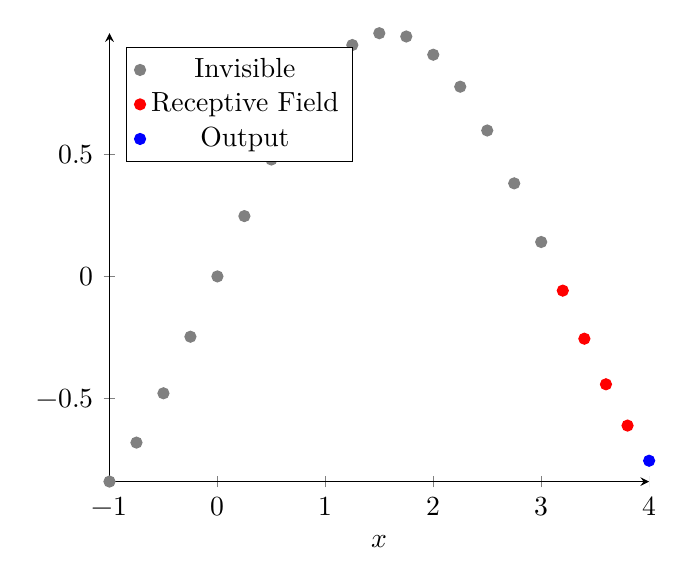
\begin{tikzpicture}
\begin{axis}[
        axis lines = left,
        xlabel = \(x\),
        domain=-10:10,
        legend pos=north west,
    ]
    \addlegendentry{Invisible}

    \addplot [
        domain=-1:3.0,
        samples=17,
        color=gray,
        only marks,
    ]
    {sin(deg(x))};

    \addplot [
        domain=3.2:3.8,
        samples=4,
        color=red,
        only marks,
    ]
    {sin(deg(x))};
    \addlegendentry{Receptive Field}

    % \addplot [
    %     domain=3.85:4.0, 
    %     samples=1, 
    %     color=blue,
    %     only marks,
    % ]
    % {sin(deg(x))};
    \addplot[color=blue,only marks]
    coordinates {
            (4.0,-0.756)
        };
    \addlegendentry{Output}
\end{axis}
\end{tikzpicture}%
\hspace{0.15cm}
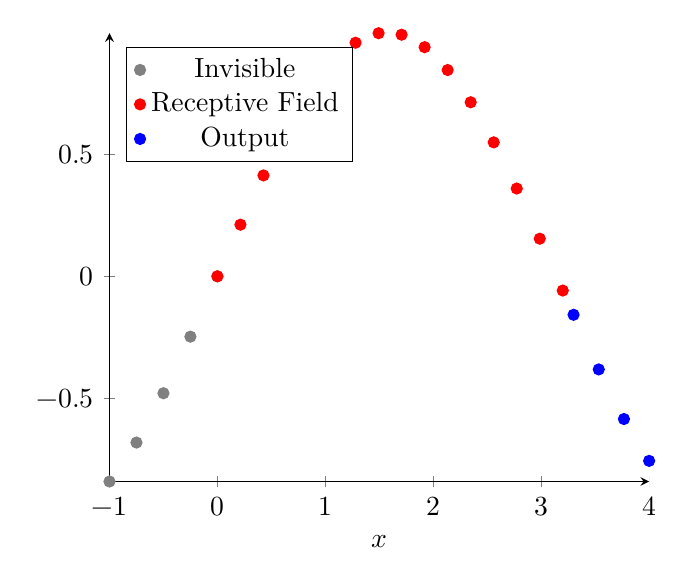
\begin{tikzpicture}
    \begin{axis}[
            axis lines = left,
            xlabel = \(x\),
            domain=-10:10,
            legend pos=north west,
        ]
        \addplot [
            domain=-1:0,
            samples=5,
            color=gray,
            only marks,
        ]
        {sin(deg(x))};
        \addlegendentry{Invisible}
        \addplot [
            domain=0:3.2,
            samples=16,
            color=red,
            only marks,
        ]
        {sin(deg(x))};
        \addlegendentry{Receptive Field}
        \addplot [
            domain=3.3:4.0,
            samples=4,
            color=blue,
            only marks,
        ]
        {sin(deg(x))};
        \addlegendentry{Output}
    \end{axis}
\end{tikzpicture}%
}
\end{figure}
\end{frame}

\begin{frame}{Expanding Receptive Field by Stacking - Results}
\protect\hypertarget{expanding-receptive-field-by-stacking---results}{}
\begin{figure}
\centering
\resizebox{!}{0.9\textheight}{
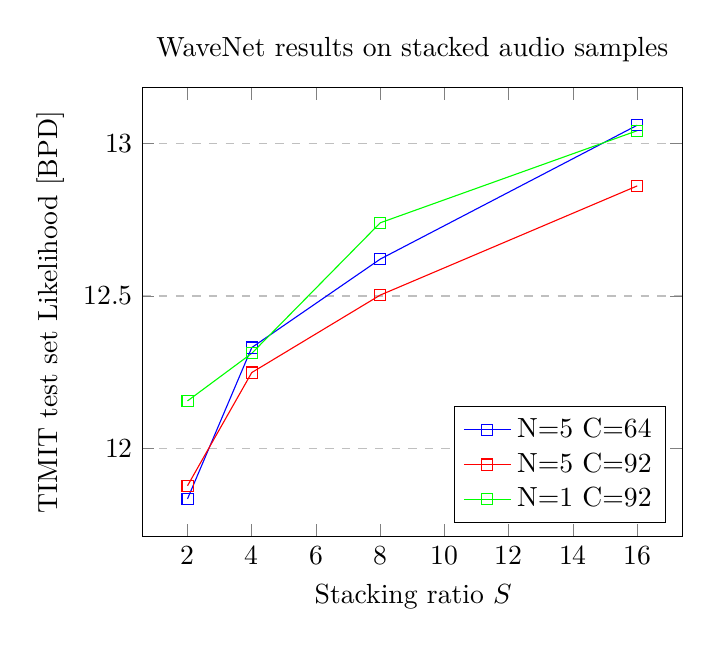
\begin{tikzpicture}
\begin{axis}[
    title={WaveNet results on stacked audio samples},
    xlabel={Stacking ratio $S$},
    ylabel={TIMIT test set Likelihood [BPD]},
    %xmin=0, xmax=16,
    %ymin=10, ymax=13,
    ymajorgrids=true,
    grid style=dashed,
    legend pos=south east,
]
\addplot[
    color=blue,
    mark=square,
    ]
    coordinates {
    (2,11.835)(4, 12.331)(8, 12.621)(16, 13.060)
    };
    \addlegendentry{N=5 C=64}
\addplot[
    color=red,
    mark=square,
    ]
    coordinates {
    (2,11.878)(4, 12.249)(8, 12.503)(16, 12.861)
    };
    \addlegendentry{N=5 C=92}

\addplot[
    color=green,
    mark=square,
    ]
    coordinates {
    (2,12.156)(4, 12.312)(8, 12.740)(16, 13.042)
    };
    \addlegendentry{N=1 C=92}
    
\end{axis}
\end{tikzpicture}
}\end{figure}
\end{frame}

\begin{frame}{Expanding Receptive Field by Stacking - Conclusions}
\protect\hypertarget{expanding-receptive-field-by-stacking---conclusions}{}
\begin{enumerate}
\tightlist
\item
  Stacking does not improve likelihoods significantly.
\item
  Increasing residual channels increases evaluation likelihoods.
\end{enumerate}

Does this mean that the WaveNet does not extract any semantic
information at all?

Is this a failure to measure the output correctly?
\end{frame}

\begin{frame}{Latent space of stacked WaveNet - Setup}
\protect\hypertarget{latent-space-of-stacked-wavenet---setup}{}
\begin{block}{Hypothesis tested}
\protect\hypertarget{hypothesis-tested-1}{}
\begin{enumerate}[<+->]
\setcounter{enumi}{1}
\tightlist
\item
  WaveNet's stacked convolutional layers learn good representations of
  speech.
\end{enumerate}
\end{block}
\end{frame}

\begin{frame}{Latent space of stacked WaveNet - Results}
\protect\hypertarget{latent-space-of-stacked-wavenet---results}{}
\begin{figure}
\includegraphics[width=0.5\columnwidth]{ 
        gfx/latent_exploration_PCA_S=2_C=64_N=5_L=10.png}%
\includegraphics[width=0.5\columnwidth]{
        gfx/latent_exploration_PCA_S=8_C=64_N=5_L=10.png
        }%
\end{figure}
\end{frame}

\begin{frame}{WaveNet as an ASR preprocessor - setup}
\protect\hypertarget{wavenet-as-an-asr-preprocessor---setup}{}
\begin{block}{Hypothesis tested}
\protect\hypertarget{hypothesis-tested-2}{}
\begin{enumerate}[<+->]
\setcounter{enumi}{1}
\tightlist
\item
  WaveNet's stacked convolutional layers learn good representations of
  speech.
\end{enumerate}
\end{block}

\begin{block}{Idea}
\protect\hypertarget{idea}{}
Are WaveNet's unsupervised representations more useful for Speech
Recognition models than raw audio?
\end{block}
\end{frame}

\begin{frame}{WaveNet as an ASR preprocessor - setup (0 layers)}
\protect\hypertarget{wavenet-as-an-asr-preprocessor---setup-0-layers}{}
\begin{figure}
\centering
\resizebox{\columnwidth}{!}{
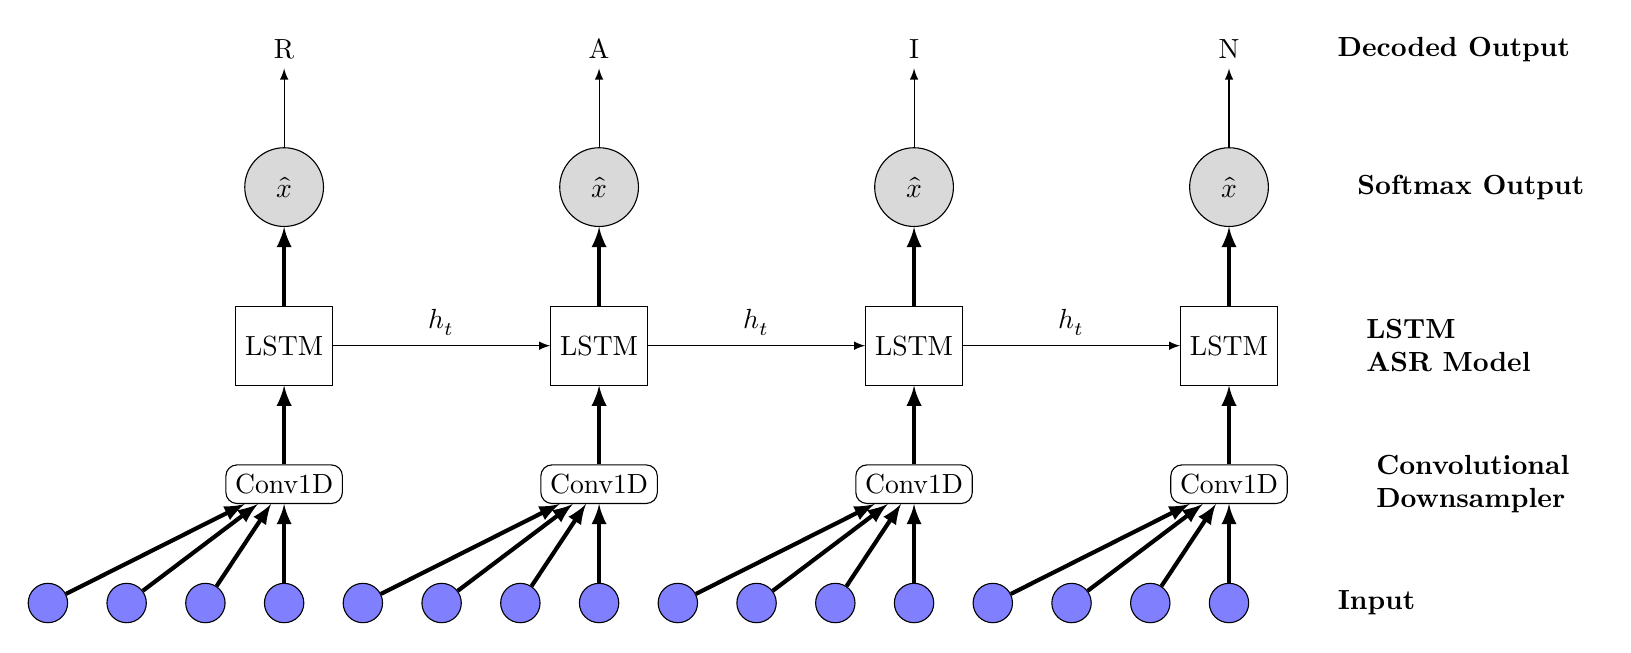
\begin{tikzpicture}
    % Input
    \foreach \x in {0, 1, ..., 15}{
            \node[circle,draw,fill=blue!50,minimum height=5mm] (Input-\x) at (\x,0) {};
        }

    %% Convolutional Layer

    \node[rectangle, draw, rounded corners, above=of Input-15] (Conv-15)  {Conv1D};
    \node[rectangle, draw, rounded corners, above=of Input-11] (Conv-11)  {Conv1D};
    \node[rectangle, draw, rounded corners, above=of Input-7] (Conv-7)  {Conv1D};
    \node[rectangle, draw, rounded corners, above=of Input-3] (Conv-3)  {Conv1D};

    \foreach \x in {0, 1, ..., 15}{
            \ifthenelse{
                \intcalcMax{\x}{3}=3
            }{
                \draw[->, line width=1.5] (Input-\x) -- (Conv-3);
            }{
                \ifthenelse{
                    \intcalcMax{\x}{7}=7
                }{
                    \draw[->, line width=1.5] (Input-\x) -- (Conv-7);
                }{
                    \ifthenelse{
                        \intcalcMax{\x}{11}=11
                    }{
                        \draw[->, line width=1.5] (Input-\x) -- (Conv-11);
                    }{

                        \draw[->, line width=1.5] (Input-\x) -- (Conv-15);
                    }
                }
            }
        }

    \foreach \i in {3,7,11,15}{
            \node[rectangle, draw, above=of Conv-\i, minimum height=1cm, minimum width=1cm] (LSTM-\i) {LSTM};
            \node[circle, minimum size = 10mm, draw, fill=gray!30, above=of LSTM-\i] (X-hat-\i) {$\hat{x}$};
            \draw[->, line width=1.5] (Conv-\i) -- (LSTM-\i);
            \draw[->, line width=1.5] (LSTM-\i) -- (X-hat-\i);
            \ifthenelse{\i=3}{!}{
                \draw[->] (LSTM-\intcalcSub{\i}{4}) -- (LSTM-\i) node[midway, above] {$h_t$};
            }
        }

    \node[above=of X-hat-3] (Text-3) {R};
    \node[above=of X-hat-7] (Text-7) {A};
    \node[above=of X-hat-11] (Text-11) {I};
    \node[above=of X-hat-15] (Text-15) {N};

    \draw[->] (X-hat-3) -- (Text-3) {};
    \draw[->] (X-hat-7) -- (Text-7) {};
    \draw[->] (X-hat-11) -- (Text-11) {};
    \draw[->] (X-hat-15) -- (Text-15) {};

    % Text and notes
    \node[right=of Input-15, align=left] {
        \textbf{Input}
    };

    \node[right=of Conv-15, align=left] {
        \textbf{Convolutional}\\\textbf{Downsampler}
    };

    \node[right=of LSTM-15, align=left] {
        \textbf{LSTM}\\\textbf{ASR Model}
    };

    \node[right=of X-hat-15, align=left] {
        \textbf{Softmax Output}
    };

    \node[right=of Text-15, align=left] {
        \textbf{Decoded Output}
    };

\end{tikzpicture}
}
\end{figure}
\end{frame}

\begin{frame}{WaveNet as an ASR preprocessor - setup (3 layers)}
\protect\hypertarget{wavenet-as-an-asr-preprocessor---setup-3-layers}{}
\begin{figure}
\centering
\resizebox{!}{0.9\textheight}{
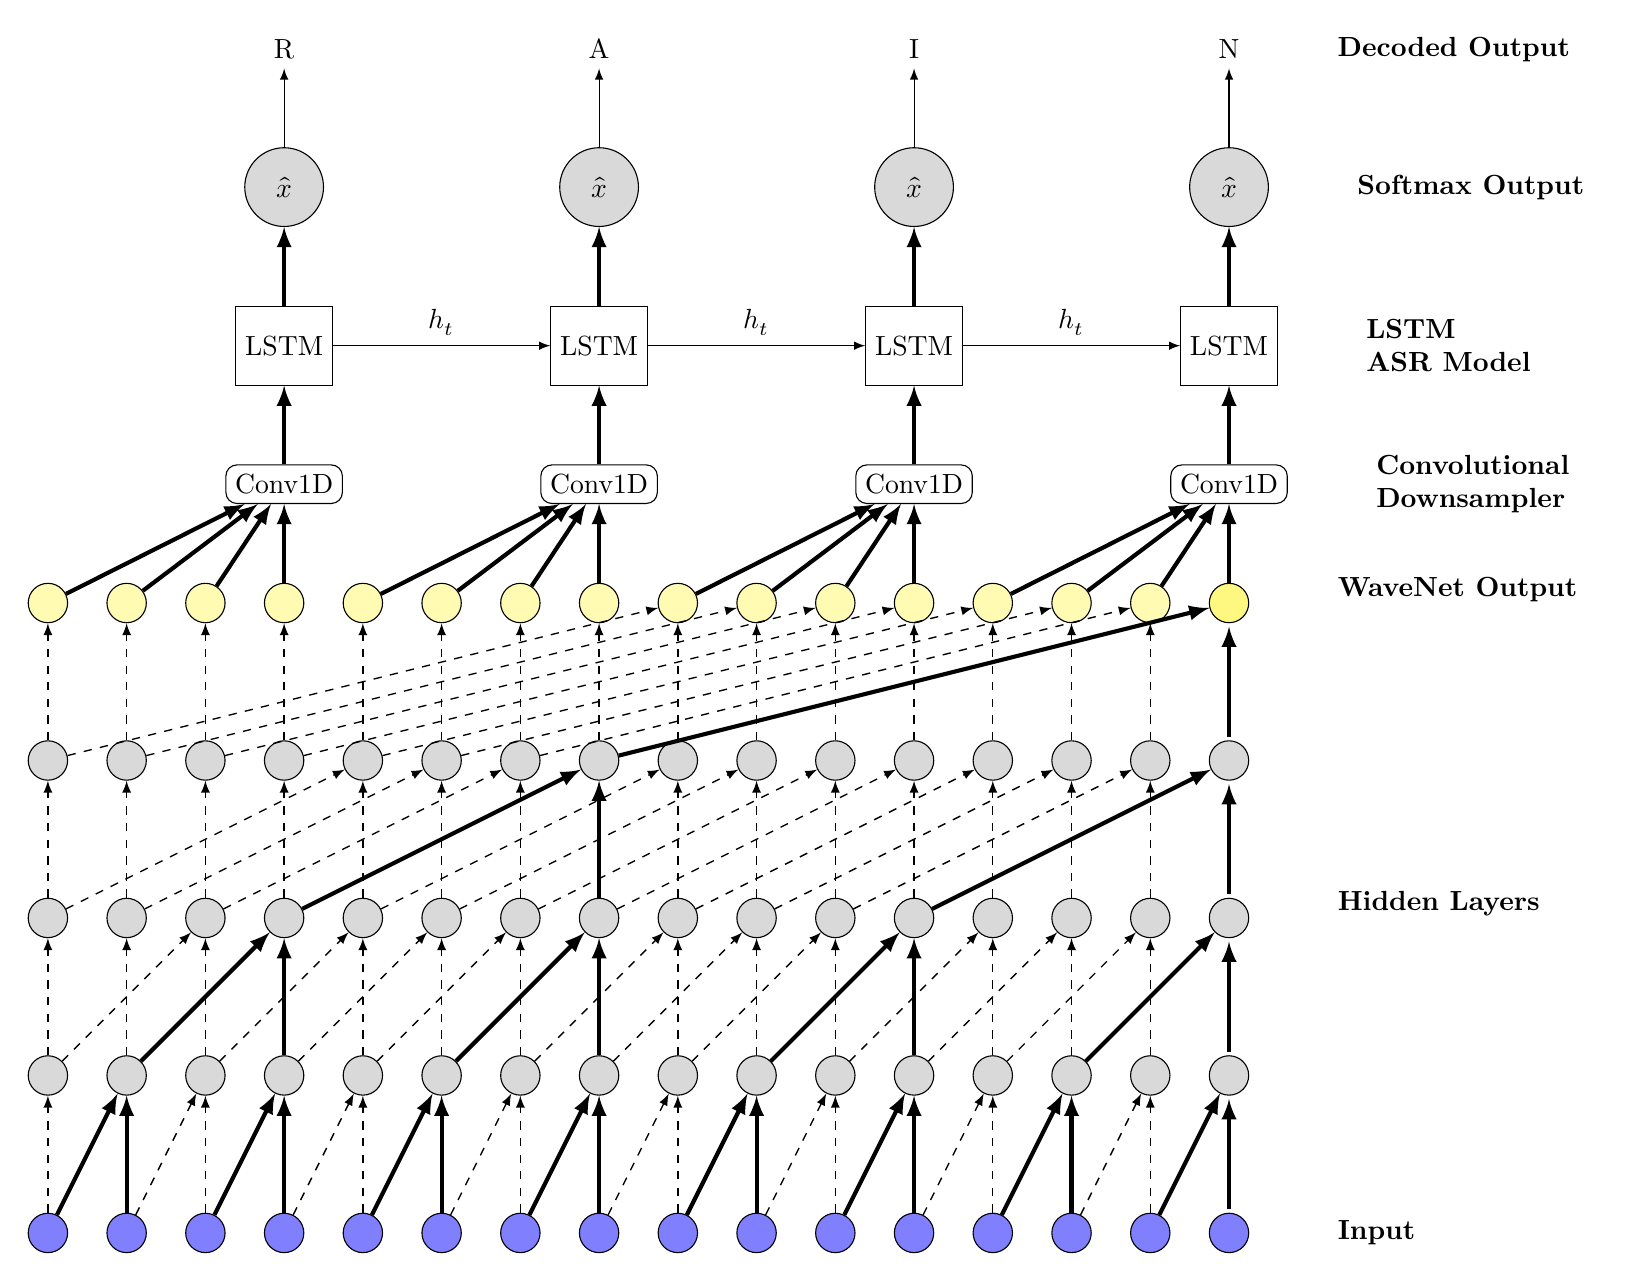
\begin{tikzpicture}
%% WaveNet Structure first


%% 


\node[circle,draw,fill=blue!50,minimum height=5mm,] (Input-15) at (15,0) {};
\node[circle,draw,fill=gray!30,minimum height=5mm, ] (Hidden1-15) at (15,2) {};
\node[circle,draw,fill=gray!30,minimum height=5mm] (Hidden2-15) at (15,4) {};
\node[circle,draw,fill=gray!30,minimum height=5mm] (Hidden3-15) at (15,6) {};
\node[circle,draw,fill=yellow!50,minimum height=5mm] (Output-15) at (15,8) {};



\draw[->, line width=1.5] (15,0.3) -- (15, 1.7);
\draw[->, line width=1.5] (15,2.3) -- (15, 3.7);
\draw[->, line width=1.5] (15,4.3) -- (15, 5.7);
\draw[->, line width=1.5] (15,6.3) -- (15, 7.7);



\foreach \x in {14, 13, ...,0}{
    \node[circle,draw,fill=blue!50,minimum height=5mm] (Input-\x) at (\x,0) {};
    \node[circle,draw,fill=gray!30,minimum height=5mm] (Hidden1-\x) at (\x,2) {};
    \node[circle,draw,fill=gray!30,minimum height=5mm] (Hidden2-\x) at (\x,4) {};
    \node[circle,draw,fill=gray!30,minimum height=5mm] (Hidden3-\x) at (\x,6) {};
    \node[circle,draw,fill=yellow!30,minimum height=5mm] (Output-\x) at (\x,8) {};
}



\foreach \x in {0, 1, ..., 14}{
	\ifthenelse{\intcalcMod{\x}{2}=0}{
		\draw[->, line width=1.5] (Input-\x) -- (Hidden1-\intcalcAdd{\x}{1});
		\draw[->, line width=.5,dashed] (Input-\x) -- (Hidden1-\x);
	}{
		\draw[->, line width=1.5] (Input-\x) -- (Hidden1-\x);
		\draw[->, line width=.5, dashed] (Input-\x) -- (Hidden1-\intcalcAdd{\x}{1});
	}
	\ifthenelse{\intcalcMod{\x}{4}=1}{
   		\draw[->, line width=1.5] (Hidden1-\x) -- (Hidden2-\intcalcAdd{\x}{2});
	}{
	    \ifnodedefined{Hidden2-\intcalcAdd{\x}{2}}{
   		\draw[->, line width=.5, dashed] (Hidden1-\x) -- (Hidden2-\intcalcAdd{\x}{2});
   		}{}
	}
	\ifthenelse{\intcalcMod{\x}{4}=3}{
   		\draw[->, line width=1.5] (Hidden1-\x) -- (Hidden2-\x);
	}{
       	\draw[->, line width=.5,dashed] (Hidden1-\x) -- (Hidden2-\x);
	}
	\ifthenelse{\intcalcMod{\x}{8}=3}{
		\draw[->, line width=1.5] (Hidden2-\x) -- (Hidden3-\intcalcAdd{\x}{4});
	}{
        \ifnodedefined{Hidden3-\intcalcAdd{\x}{4}}{
   		    \draw[->, line width=.5, dashed] (Hidden2-\x) -- (Hidden3-\intcalcAdd{\x}{4});
   		}{}
	}
	\ifthenelse{\intcalcMod{\x}{8}=7}{
   		\draw[->, line width=1.5] (Hidden2-\x) -- (Hidden3-\x);
	}{
   		\draw[->, line width=.5, dashed] (Hidden2-\x) -- (Hidden3-\x);
	}
	\ifthenelse{\intcalcMod{\x}{16}=7}{
		\draw[->, line width=1.5] (Hidden3-\x) -- (Output-\intcalcAdd{\x}{8});
	}{
	\ifnodedefined{Output-\intcalcAdd{\x}{8}}{
   		    \draw[->, line width=.5, dashed] (Hidden3-\x) -- (Output-\intcalcAdd{\x}{8});
   		}{}
	}
	\ifthenelse{\intcalcMod{\x}{16}=15}{
   		\draw[->, line width=1.5] (Hidden3-\x) -- (Output-\x);
	}{
	\draw[->,  line width=.5, dashed] (Hidden3-\x) -- (Output-\x);
	}
}



%% Convolutional Layer

\node[rectangle, draw, rounded corners, above=of Output-15] (Conv-15)  {Conv1D};
\node[rectangle, draw, rounded corners, above=of Output-11] (Conv-11)  {Conv1D};
\node[rectangle, draw, rounded corners, above=of Output-7] (Conv-7)  {Conv1D};
\node[rectangle, draw, rounded corners, above=of Output-3] (Conv-3)  {Conv1D};

\foreach \x in {0, 1, ..., 15}{
\ifthenelse{
    \intcalcMax{\x}{3}=3
}{
    \draw[->, line width=1.5] (Output-\x) -- (Conv-3);
}{
\ifthenelse{
    \intcalcMax{\x}{7}=7
}{
    \draw[->, line width=1.5] (Output-\x) -- (Conv-7);
}{
\ifthenelse{
    \intcalcMax{\x}{11}=11
}{
    \draw[->, line width=1.5] (Output-\x) -- (Conv-11);
}{

    \draw[->, line width=1.5] (Output-\x) -- (Conv-15);
}
}
}
}

\foreach \i in {3,7,11,15}{
\node[rectangle, draw, above=of Conv-\i, minimum height=1cm, minimum width=1cm] (LSTM-\i) {LSTM};
\node[circle, minimum size = 10mm, draw, fill=gray!30, above=of LSTM-\i] (X-hat-\i) {$\hat{x}$};
\draw[->, line width=1.5] (Conv-\i) -- (LSTM-\i);
\draw[->, line width=1.5] (LSTM-\i) -- (X-hat-\i);
\ifthenelse{\i=3}{!}{
\draw[->] (LSTM-\intcalcSub{\i}{4}) -- (LSTM-\i) node[midway, above] {$h_t$};
}
}


\node[above=of X-hat-3] (Text-3) {R};
\node[above=of X-hat-7] (Text-7) {A};
\node[above=of X-hat-11] (Text-11) {I};
\node[above=of X-hat-15] (Text-15) {N};

\draw[->] (X-hat-3) -- (Text-3) {};
\draw[->] (X-hat-7) -- (Text-7) {};
\draw[->] (X-hat-11) -- (Text-11) {};
\draw[->] (X-hat-15) -- (Text-15) {};

% Text and notes
\node[right=of Input-15, align=left] {
\textbf{Input}
};
% \node[right=of Hidden1-15, align=left] {
% \textbf{Hidden1}\\
% Dilation = 1
% };
\node[right=of Hidden2-15, align=left] {
\textbf{Hidden Layers}\\
};
% \node[right=of Hidden3-15, align=left] {
% \textbf{Hidden3}\\
% Dilation = 4
% };
\node[right=of Output-15, align=left] {
\textbf{WaveNet Output}\\
};

\node[right=of Conv-15, align=left] {
\textbf{Convolutional}\\\textbf{Downsampler}
};

\node[right=of LSTM-15, align=left] {
\textbf{LSTM}\\\textbf{ASR Model}
};

\node[right=of X-hat-15, align=left] {
\textbf{Softmax Output}
};

\node[right=of Text-15, align=left] {
\textbf{Decoded Output}
};

\end{tikzpicture}
}
\end{figure}
\end{frame}

\begin{frame}{WaveNet as an ASR preprocessor - Results}
\protect\hypertarget{wavenet-as-an-asr-preprocessor---results}{}
\begin{figure}
\centering
\resizebox{!}{\textheight}{
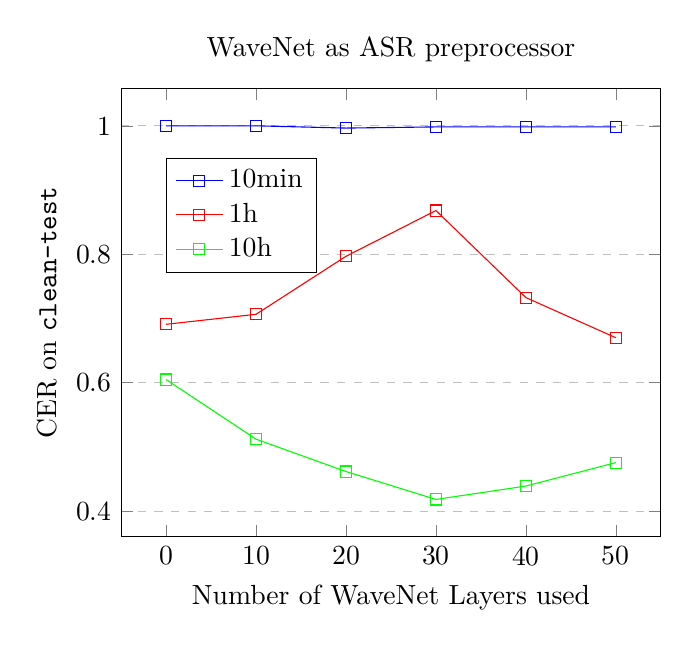
\begin{tikzpicture}
\begin{axis}[
    title={WaveNet as ASR preprocessor},
    xlabel={Number of WaveNet Layers used},
    ylabel={CER on \texttt{clean-test}},
    ymajorgrids=true,
    grid style=dashed,
    legend style={at={(axis cs:0,0.95)},anchor=north west},
    legend cell align={left},
]
\addplot[
    color=blue,
    mark=square,
    ]
    coordinates {
    (0,1.00)(10, 1.0)(20, 0.9965)(30, 0.9983)(40, 0.9983)(50, 0.9983)
    };
    \addlegendentry{10min}
\addplot[
    color=red,
    mark=square,
    ]
    coordinates {
    (0,0.691)(10,0.7066)(20, 0.7969)(30, 0.8681)(40, 0.7326)(50, 0.6701)
    };
    \addlegendentry{1h}

\addplot[
    color=green,
    mark=square,
    ]
    coordinates {
    (0,0.6050)(10,0.5122)(20, 0.4618)(30, 0.4184)(40, 0.4392)(50, 0.4757)
    };
    \addlegendentry{10h}
    
\end{axis}
\end{tikzpicture}
}\end{figure}
\end{frame}

\begin{frame}{WaveNet as an ASR preprocessor - Conclusions}
\protect\hypertarget{wavenet-as-an-asr-preprocessor---conclusions}{}
\begin{itemize}
\item
  Using WaveNet as a preprocessor decreases the loss when trained on the
  1 hour and 10-hour training subsets.
\item
  The best performance occurs when using 30 layers of the WaveNet
  trained on 10 hours of training data.
\item
  Notably, WaveNet's use as a preprocessor grows more competitive when
  increasing the training data size.
\end{itemize}
\end{frame}

\begin{frame}{WaveNet as a Language Model - Setup}
\protect\hypertarget{wavenet-as-a-language-model---setup}{}
\begin{block}{Hypothesis tested}
\protect\hypertarget{hypothesis-tested-3}{}
\begin{enumerate}[<+->]
\setcounter{enumi}{2}
\tightlist
\item
  WaveNet's hierarchical structure makes it suitable to learn priors
  over representations of speech such as text.
\end{enumerate}
\end{block}

\begin{block}{Setup}
\protect\hypertarget{setup-1}{}
\end{block}
\end{frame}

\begin{frame}{WaveNet as a Language Model - Results}
\protect\hypertarget{wavenet-as-a-language-model---results}{}
\begin{table}[htb]
    \centering
    \begin{tabular}{l|c||c}
        Model & Dataset & BPD (test) \\
        \hline
        Mogrifier LSTM \cite{melis_mogrifier_2020} & PTB & 1.083 \\
        Temporal Convolutional Network \cite{bai_empirical_2018} & PTB & 1.31 \\
        \hline
        WaveNet N=5 L=4 R=24 [RF 126] & PTB & 1.835 \\
        WaveNet N=5 L=4 R=32 [RF 126] & PTB & \textbf{1.666} \\
        WaveNet N=5 L=4 R=48 [RF 126] & PTB & 1.678 \\
        % WaveNet L=4 N=5 R=64 [RF 126] & Billion Word & 1.483 \\%1.677 \\
    \end{tabular}
\end{table}
\end{frame}

\begin{frame}{WaveNet as a Language Model - Conclusions}
\protect\hypertarget{wavenet-as-a-language-model---conclusions}{}
\end{frame}

\hypertarget{conclusions}{%
\section{Conclusions}\label{conclusions}}

\begin{frame}{Conclusions}
\begin{longtable}[]{@{}ll@{}}
\toprule
\begin{minipage}[b]{0.83\columnwidth}\raggedright
Hypothesis\strut
\end{minipage} & \begin{minipage}[b]{0.11\columnwidth}\raggedright
Support?\strut
\end{minipage}\tabularnewline
\midrule
\endhead
\begin{minipage}[t]{0.83\columnwidth}\raggedright
WaveNet's receptive field is the main limiting factor for modeling
long-range dependencies.\strut
\end{minipage} & \begin{minipage}[t]{0.11\columnwidth}\raggedright
No\strut
\end{minipage}\tabularnewline
\begin{minipage}[t]{0.83\columnwidth}\raggedright
WaveNet's stacked convolutional layers learn good representations of
speech.\strut
\end{minipage} & \begin{minipage}[t]{0.11\columnwidth}\raggedright
Yes\strut
\end{minipage}\tabularnewline
\begin{minipage}[t]{0.83\columnwidth}\raggedright
WaveNet's hierarchical structure makes it suitable to learn priors over
representations of speech such as text.\strut
\end{minipage} & \begin{minipage}[t]{0.11\columnwidth}\raggedright
No\strut
\end{minipage}\tabularnewline
\begin{minipage}[t]{0.83\columnwidth}\raggedright
A large WaveNet architecture trained on speech can generate coherent
words and sentence fragments\strut
\end{minipage} & \begin{minipage}[t]{0.11\columnwidth}\raggedright
No\strut
\end{minipage}\tabularnewline
\bottomrule
\end{longtable}
\end{frame}

\begin{frame}{References}
\protect\hypertarget{references}{}
\bibliography{vseq}
\bibliographystyle{abbrv}
\end{frame}

\hypertarget{appendix-slides}{%
\section{Appendix Slides}\label{appendix-slides}}

\begin{frame}[fragile]{Experiment: WaveNet Gradient analysis over input
space - 1}
\protect\hypertarget{experiment-wavenet-gradient-analysis-over-input-space---1}{}
\begin{block}{Explained}
\protect\hypertarget{explained}{}
Run gradient evaluation over a trained WaveNet model and visualize the
outputs.
\end{block}

\begin{block}{Hypothesis tested}
\protect\hypertarget{hypothesis-tested-4}{}
\textbf{WaveNet uses the entirety of its receptive field for next-step
prediction.}

\begin{itemize}
\item
  Gradients in the end of the RF (close to output) are larger than the
  gradients in the rest of the RF.
\item
  Gradients do NOT collapse to 0 around the beginning of the RF
  (furthest away from output).
\end{itemize}
\end{block}

\begin{block}{Method}
\protect\hypertarget{method}{}
\begin{enumerate}
\tightlist
\item
  Calculate vector-Jacobian product with \texttt{torch.autograd}
\item
  Calculate norm with \texttt{torch.linalg.norm}
\end{enumerate}
\end{block}
\end{frame}

\begin{frame}{Experiment: WaveNet Gradient analysis over input space -
2}
\protect\hypertarget{experiment-wavenet-gradient-analysis-over-input-space---2}{}
\begin{figure}[ht]
%        \resizebox{\columnwidth}{!}{
            \includegraphics[width=0.49\textwidth]{gfx/wavenet-8-4-64-epoch-70-gradients.png}%
            \includegraphics[width=0.49\textwidth]{gfx/wavenet-8-4-64-epoch-70-gradients-zoom.png}
 %       }
\end{figure}
\end{frame}

\begin{frame}{Notation}
\protect\hypertarget{notation}{}
\begin{longtable}[]{@{}ll@{}}
\toprule
\begin{minipage}[b]{0.32\columnwidth}\raggedright
Symbol\strut
\end{minipage} & \begin{minipage}[b]{0.62\columnwidth}\raggedright
Explanation\strut
\end{minipage}\tabularnewline
\midrule
\endhead
\begin{minipage}[t]{0.32\columnwidth}\raggedright
\(x_i\),\(x_t\)\strut
\end{minipage} & \begin{minipage}[t]{0.62\columnwidth}\raggedright
The \(i\)th index of \(\mathbf{x}\), of size \(N\).
\(x_i \in \mathbb{R}^N\). \(x_t\) is used when data is
time-resolved.\strut
\end{minipage}\tabularnewline
\begin{minipage}[t]{0.32\columnwidth}\raggedright
\(\mathbf{x}\)\strut
\end{minipage} & \begin{minipage}[t]{0.62\columnwidth}\raggedright
The data x, composed of vectors \(x_i\).
\(\mathbf{x} \in \mathbb{R}^{T \times N}\)\strut
\end{minipage}\tabularnewline
\begin{minipage}[t]{0.32\columnwidth}\raggedright
\(p_\theta(\cdot )\), \(p(\cdot )\)\strut
\end{minipage} & \begin{minipage}[t]{0.62\columnwidth}\raggedright
Likelihood function over model parameters \(\theta\). Denoted
\(p(\cdot )\) for brevity\strut
\end{minipage}\tabularnewline
\begin{minipage}[t]{0.32\columnwidth}\raggedright
\(\hat{x}_i\)\strut
\end{minipage} & \begin{minipage}[t]{0.62\columnwidth}\raggedright
Model prediction for \(x_i\).\strut
\end{minipage}\tabularnewline
\begin{minipage}[t]{0.32\columnwidth}\raggedright
\(\mathcal{L}_{i}\)\strut
\end{minipage} & \begin{minipage}[t]{0.62\columnwidth}\raggedright
Loss function for \(i\)th index.\strut
\end{minipage}\tabularnewline
\begin{minipage}[t]{0.32\columnwidth}\raggedright
\(R\)\strut
\end{minipage} & \begin{minipage}[t]{0.62\columnwidth}\raggedright
Receptive field size.\strut
\end{minipage}\tabularnewline
\begin{minipage}[t]{0.32\columnwidth}\raggedright
\(S\)\strut
\end{minipage} & \begin{minipage}[t]{0.62\columnwidth}\raggedright
Size of stack size used in stack transformations\strut
\end{minipage}\tabularnewline
\begin{minipage}[t]{0.32\columnwidth}\raggedright
\(d_i\)\strut
\end{minipage} & \begin{minipage}[t]{0.62\columnwidth}\raggedright
Dilation of \(i\)th layer in a WaveNet architecture\strut
\end{minipage}\tabularnewline
\begin{minipage}[t]{0.32\columnwidth}\raggedright
\(C\)\strut
\end{minipage} & \begin{minipage}[t]{0.62\columnwidth}\raggedright
Number of residual channels\strut
\end{minipage}\tabularnewline
\bottomrule
\end{longtable}
\end{frame}

\begin{frame}{Overview of Codebase}
\protect\hypertarget{overview-of-codebase}{}
\begin{columns}[T]
\begin{column}{0.48\textwidth}
\begin{itemize}
\tightlist
\item
  Collaborative codebase with Jakob Havtorn and Lasse Borgholt (PhDs at
  Corti)
\item
  Includes custom implementations of many modules in the
\end{itemize}
\end{column}

\begin{column}{0.48\textwidth}
TODO: Implementations to mention:

\begin{itemize}
\tightlist
\item
  Residual Stack
\item
  Categorical WaveNet
\item
  DMoL WaveNet
\end{itemize}
\end{column}
\end{columns}
\end{frame}

\begin{frame}{Stacking Transformation}
\protect\hypertarget{stacking-transformation}{}
\[
x^*_t = \begin{pmatrix}
        x_{t} \\ \vdots \\ x_{t+S} \\
    \end{pmatrix},
    \hspace{1cm}
    t\in\{1,S+1,\dots,T-S\}, \mathbf{x}^*\in\mathbb{R}^{N/S \times S}\mathbf{x}\in\mathbb{R}^{N}
\]
\end{frame}

\begin{frame}{Residual Block of WaveNet}
\protect\hypertarget{residual-block-of-wavenet}{}
\begin{figure}
    \centering
    \resizebox{!}{0.9\textheight}{
    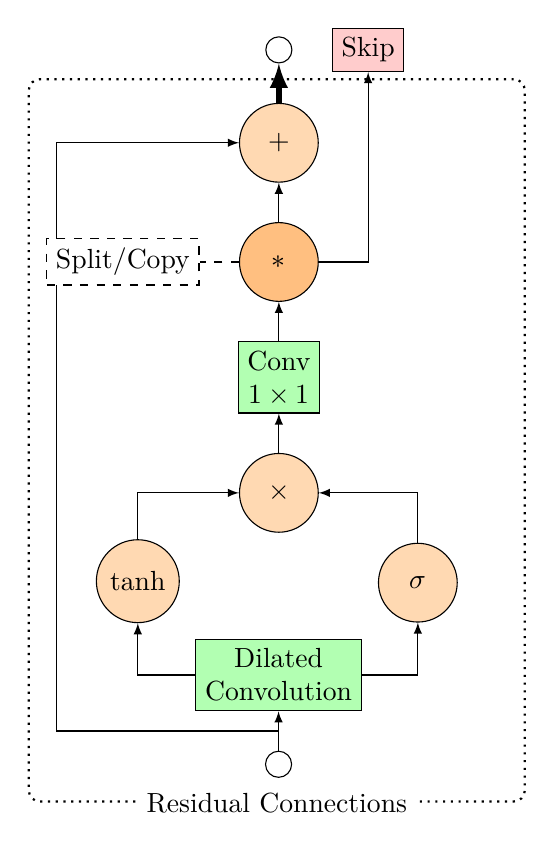
\begin{tikzpicture}[  node distance = 5mm,]
    %[transform canvas={scale=0.5}]
    % \tikzset{
    %     myarrow/.style={->, >=latex', shorten >=1pt, thick},
    % }

    % Inside res stack
    % Input node

    \node[circle, minimum size = 3mm,draw,% fill=orange!30,
    ] (Res-Input) at (0,0) {};


    \node[rectangle,
        fill=green!30,draw,
        above=of Res-Input,
        align=center] (Dilated-Conv) {Dilated \\ Convolution};

    \path (Res-Input.north) -- node (Res-Empty-Input-Conv) {} (Dilated-Conv.south);

    \node[circle,
        minimum size = 10mm,
        draw,
        fill=orange!30,
        above right=of Dilated-Conv,
    ] (Res-Sigmoid) {$\sigma$};

    \node[circle,
        minimum size = 10mm,
        draw,
        fill=orange!30,
        above left=of Dilated-Conv,
    ] (Res-Tanh) {tanh};

    % invisible node in middle 

    \path (Res-Tanh.east) -- node (Res-Empty-Res-Sigmoid) {} (Res-Sigmoid.west);


    \node[circle,
        minimum size = 10mm,
        draw,
        fill=orange!30,
        above=of Res-Empty-Res-Sigmoid,
    ] (Res-Multiply) {$\times$};


    \node[rectangle, fill=green!30,draw, above=of Res-Multiply, align=center] (Res-1x1) {Conv\\$1 \times 1$};
    \node[circle, fill=orange!50,draw, minimum size = 10mm, above=of Res-1x1, align=center] (Res-Split) {$*$};
    \node[circle,
        minimum size = 10mm,
        draw,
        fill=orange!30,
        above=of Res-Split,
    ] (Res-Add) {$+$};

    \node[circle, minimum size = 3mm,draw,above=of Res-Add] (Res-Add-Output) {};

    \node[rectangle, fill=red!20,draw, right=of Res-Add-Output, align=center] (Res-Skip) {Skip};

    \coordinate[left=of Res-Tanh] (a);
    \coordinate[right=of Res-Sigmoid] (b);


    % ARROWS
    \draw[->] (Res-Input) -- (Dilated-Conv);
    \draw[->] (Dilated-Conv) -| (Res-Tanh);
    \draw[->] (Dilated-Conv) -| (Res-Sigmoid);

    \draw[->] (Res-Tanh) |- (Res-Multiply);
    \draw[->] (Res-Sigmoid) |- (Res-Multiply);

    \draw[->] (Res-Multiply) -- (Res-1x1);
    % \draw[->] (Res-1x1) -- (Res-Add) ;	

    \draw[->] (Res-1x1) -- (Res-Split) ;

    \draw[->] (Res-Split) -| (Res-Skip) ;
    \draw[->] (Res-Split) -- (Res-Add) ;

    \draw[->] (Res-Empty-Input-Conv.center) -| (a)  |- (Res-Add);
    \draw[->, line width=2] (Res-Add) -- (Res-Add-Output);


    \node[fill=white, left=of Res-Split, align=center, draw, dashed] (Res-Split-Label) {Split/Copy};
    \draw[dashed] (Res-Split) -- (Res-Split-Label);
    %%% RECTANGLE AROUND ALL 

    \node[draw, thick, dotted, rounded corners, inner xsep=1em, inner ysep=3mm, fit=(Res-Input) (a) (b) (Res-Add)] (box) {};
    \node[fill=white] at (box.south) {Residual Connections};


\end{tikzpicture}
    %\caption{
    %Overview of WaveNet's residual block. 
    %The "Split/Copy" operation, representing the two configurations of the residual block is highlighted.
    %}
    %\label{fig:wavenet-res-block}
   }
\end{figure}
\end{frame}

\begin{frame}{Full WaveNet architecture}
\protect\hypertarget{full-wavenet-architecture}{}
\begin{figure}
    \centering
    \resizebox{!}{0.9\textheight}{
    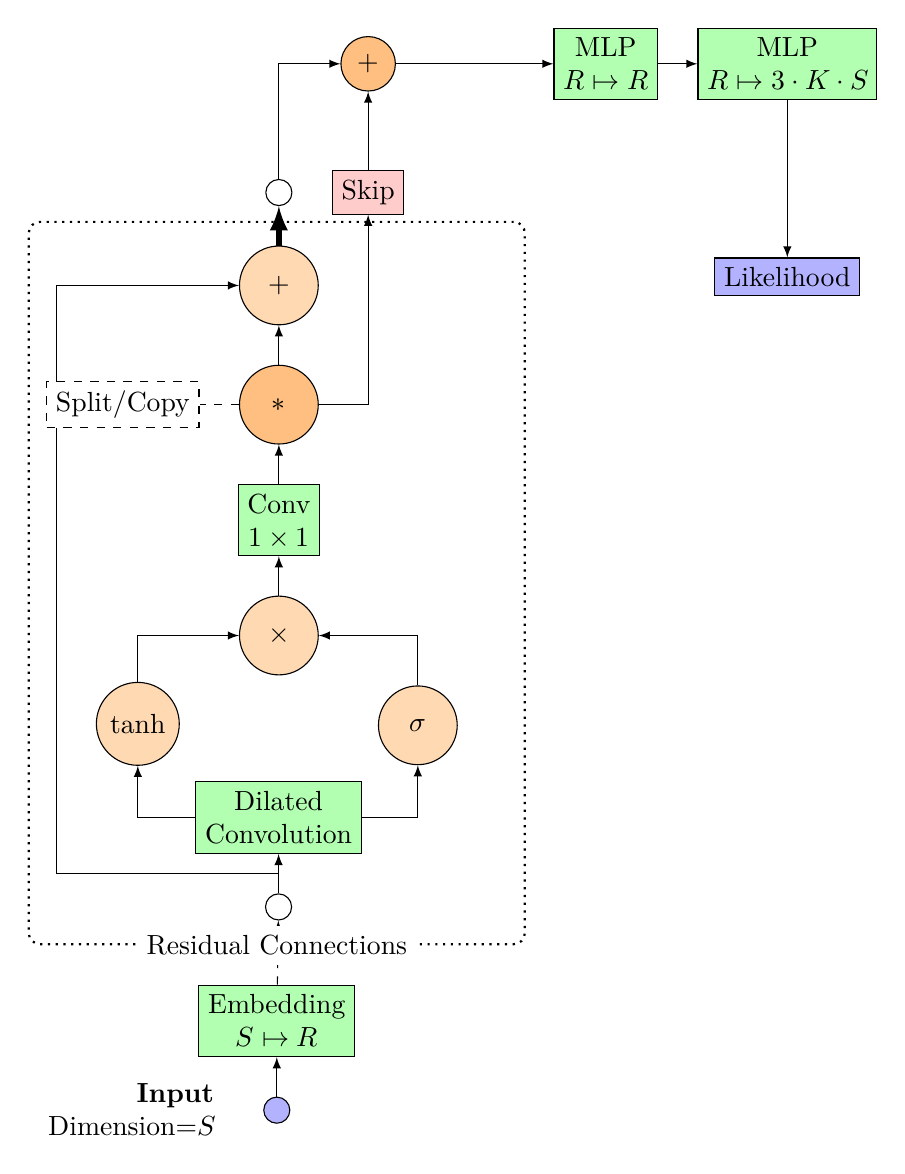
\begin{tikzpicture}[  node distance = 5mm,]
    %[transform canvas={scale=0.5}]
    % \tikzset{
    %     myarrow/.style={->, >=latex', shorten >=1pt, thick},
    % }

    % Inside res stack
    % Input node

    \node[circle, minimum size = 3mm,draw,% fill=orange!30,
    ] (Res-Input) at (0,0) {};


    \node[rectangle,
        fill=green!30,draw,
        above=of Res-Input,
        align=center] (Dilated-Conv) {Dilated \\ Convolution};

    \path (Res-Input.north) -- node (Res-Empty-Input-Conv) {} (Dilated-Conv.south);

    \node[circle,
        minimum size = 10mm,
        draw,
        fill=orange!30,
        above right=of Dilated-Conv,
    ] (Res-Sigmoid) {$\sigma$};

    \node[circle,
        minimum size = 10mm,
        draw,
        fill=orange!30,
        above left=of Dilated-Conv,
    ] (Res-Tanh) {tanh};

    % invisible node in middle 

    \path (Res-Tanh.east) -- node (Res-Empty-Res-Sigmoid) {} (Res-Sigmoid.west);


    \node[circle,
        minimum size = 10mm,
        draw,
        fill=orange!30,
        above=of Res-Empty-Res-Sigmoid,
    ] (Res-Multiply) {$\times$};


    \node[rectangle, fill=green!30,draw, above=of Res-Multiply, align=center] (Res-1x1) {Conv\\$1 \times 1$};
    \node[circle, fill=orange!50,draw, minimum size = 10mm, above=of Res-1x1, align=center] (Res-Split) {$*$};
    \node[circle,
        minimum size = 10mm,
        draw,
        fill=orange!30,
        above=of Res-Split,
    ] (Res-Add) {$+$};

    \node[circle, minimum size = 3mm,draw,above=of Res-Add] (Res-Add-Output) {};

    \node[rectangle, fill=red!20,draw, right=of Res-Add-Output, align=center] (Res-Skip) {Skip};

    \coordinate[left=of Res-Tanh] (a);
    \coordinate[right=of Res-Sigmoid] (b);


    % ARROWS
    \draw[->] (Res-Input) -- (Dilated-Conv);
    \draw[->] (Dilated-Conv) -| (Res-Tanh);
    \draw[->] (Dilated-Conv) -| (Res-Sigmoid);

    \draw[->] (Res-Tanh) |- (Res-Multiply);
    \draw[->] (Res-Sigmoid) |- (Res-Multiply);

    \draw[->] (Res-Multiply) -- (Res-1x1);
    % \draw[->] (Res-1x1) -- (Res-Add) ;	

    \draw[->] (Res-1x1) -- (Res-Split) ;

    \draw[->] (Res-Split) -| (Res-Skip) ;
    \draw[->] (Res-Split) -- (Res-Add) ;

    \draw[->] (Res-Empty-Input-Conv.center) -| (a)  |- (Res-Add);
    \draw[->, line width=2] (Res-Add) -- (Res-Add-Output);


    \node[fill=white, left=of Res-Split, align=center, draw, dashed] (Res-Split-Label) {Split/Copy};
    \draw[dashed] (Res-Split) -- (Res-Split-Label);
    %%% RECTANGLE AROUND ALL 

    \node[draw, thick, dotted, rounded corners, inner xsep=1em, inner ysep=3mm, fit=(Res-Input) (a) (b) (Res-Add)] (box) {};



    %% Input 
    \node[rectangle, draw, below=of box.south, fill=green!30,align=center] (Outside-Embedding) {Embedding\\$S\mapsto R$};
    
    
    \node[circle, draw, below=of Outside-Embedding, minimum size= 3mm, fill=blue!30,] (Outside-Input) {};
    \draw[->, dashed] (Outside-Embedding) -- (Res-Input);
    \draw[->,] (Outside-Input) -- (Outside-Embedding);
    

\node[left=of Outside-Input, align=right] {
\textbf{Input}\\
Dimension=$S$
};


    % red conn label here    
    \node[fill=white] at (box.south) {Residual Connections};

    
    %% Output
    \node[circle, draw, above=1cm of Res-Skip, minimum size= 3mm, fill=orange!50,] (Outside-Sum) {$+$};

    \draw[->] (Res-Skip) -- (Outside-Sum) ;
    \draw[->] (Res-Add-Output) |- (Outside-Sum) ;
        
    \node[rectangle, fill=green!30,draw, right=2cm of Outside-Sum, align=center] (Output-Transform) {MLP\\$R \mapsto R$};
    \node[rectangle, fill=green!30,draw, right=of Output-Transform, align=center] (LLH-Transform) {MLP\\$R \mapsto 3\cdot K\cdot S$};

    \draw[->] (Outside-Sum) -- (Output-Transform) ;
    \draw[->] (Output-Transform) -- (LLH-Transform) ;

    \node[rectangle, fill=blue!30,draw, below=2 cm of LLH-Transform, align=center] (LLH) {Likelihood};
    \draw[->] (LLH-Transform) -- (LLH) ;

\end{tikzpicture}
   }
\end{figure}
\end{frame}

\begin{frame}{DMoL vs.~Categorical output distribution}
\protect\hypertarget{dmol-vs.-categorical-output-distribution}{}
\begin{block}{Discretized Mixture of Logistics}
\protect\hypertarget{discretized-mixture-of-logistics}{}
With a mixture of \(K\) logistic distributions, for all discrete values
of \(x\) except edge cases: \[
P(x|\pi, \mu, s) =CDF(x-0.5, x+0.5) = \sum_{i=1}^K \pi_i[\sigma(\frac{x +0.5 - \mu_i}{s_i}) - \sigma(\frac{x-0.5-\mu_i}{s_i}) ]
\] Where \(\sigma(\cdot )\) is the logistic sigmoid:
\(\sigma(x) = \frac{1}{1+e^x}\), \(\pi\) is the relative weight vector,
\(\mu\) is the location vector and \(s\) is the scale vector.
\end{block}

\begin{block}{Softmax distribution}
\protect\hypertarget{softmax-distribution}{}
In a softmax distribution, the probability of the \(i\)th out of N
discrete values is defined by: \[
\sigma(\mathbf{x})_i = \frac{\exp(x_i)}{\sum_{j=1}^N \exp(x_j)}
\]
\end{block}
\end{frame}

\begin{frame}{Different tested embeddings for stacked WaveNet input}
\protect\hypertarget{different-tested-embeddings-for-stacked-wavenet-input}{}
\begin{longtable}[]{@{}llll@{}}
\toprule
\begin{minipage}[b]{0.39\columnwidth}\raggedright
Embedding type\strut
\end{minipage} & \begin{minipage}[b]{0.03\columnwidth}\raggedright
Dim\strut
\end{minipage} & \begin{minipage}[b]{0.08\columnwidth}\raggedright
Number\strut
\end{minipage} & \begin{minipage}[b]{0.39\columnwidth}\raggedright
Note\strut
\end{minipage}\tabularnewline
\midrule
\endhead
\begin{minipage}[t]{0.39\columnwidth}\raggedright
Lookup table embedding with input dimensionality \(S\times C\)\strut
\end{minipage} & \begin{minipage}[t]{0.03\columnwidth}\raggedright
\(128\)\strut
\end{minipage} & \begin{minipage}[t]{0.08\columnwidth}\raggedright
\(1024\)\strut
\end{minipage} & \begin{minipage}[t]{0.39\columnwidth}\raggedright
Outputs collapsed to silence (suspect too sparse embeddings)\strut
\end{minipage}\tabularnewline
\begin{minipage}[t]{0.39\columnwidth}\raggedright
\(S\) embeddings convolved together\strut
\end{minipage} & \begin{minipage}[t]{0.03\columnwidth}\raggedright
128\strut
\end{minipage} & \begin{minipage}[t]{0.08\columnwidth}\raggedright
\(S\cdot 256\)\strut
\end{minipage} & \begin{minipage}[t]{0.39\columnwidth}\raggedright
White noise output.\strut
\end{minipage}\tabularnewline
\begin{minipage}[t]{0.39\columnwidth}\raggedright
2 Layer perceptron with input size \(S\) and output size \(R\)\strut
\end{minipage} & \begin{minipage}[t]{0.03\columnwidth}\raggedright
\(R\)\strut
\end{minipage} & \begin{minipage}[t]{0.08\columnwidth}\raggedright
Continuous\strut
\end{minipage} & \begin{minipage}[t]{0.39\columnwidth}\raggedright
Final used embedding\strut
\end{minipage}\tabularnewline
\bottomrule
\end{longtable}
\end{frame}

\begin{frame}{Overview of extra experiments}
\protect\hypertarget{overview-of-extra-experiments}{}
\begin{longtable}[]{@{}lll@{}}
\toprule
\begin{minipage}[b]{0.26\columnwidth}\raggedright
Model\strut
\end{minipage} & \begin{minipage}[b]{0.35\columnwidth}\raggedright
Dataset(s)\strut
\end{minipage} & \begin{minipage}[b]{0.30\columnwidth}\raggedright
Notes\strut
\end{minipage}\tabularnewline
\midrule
\endhead
\begin{minipage}[t]{0.26\columnwidth}\raggedright
Single-Timestep WaveNet (softmax output)\strut
\end{minipage} & \begin{minipage}[t]{0.35\columnwidth}\raggedright
TIMIT\strut
\end{minipage} & \begin{minipage}[t]{0.30\columnwidth}\raggedright
Slow convergence compared to later DMoL\strut
\end{minipage}\tabularnewline
\begin{minipage}[t]{0.26\columnwidth}\raggedright
Stacked WaveNet (softmax output)\strut
\end{minipage} & \begin{minipage}[t]{0.35\columnwidth}\raggedright
TIMIT, Librispeech\strut
\end{minipage} & \begin{minipage}[t]{0.30\columnwidth}\raggedright
Collapses to predict silence for all timesteps\strut
\end{minipage}\tabularnewline
\begin{minipage}[t]{0.26\columnwidth}\raggedright
Single Timestep WaveNet\strut
\end{minipage} & \begin{minipage}[t]{0.35\columnwidth}\raggedright
Generated Sinusoids with periodically modulated pitch.\strut
\end{minipage} & \begin{minipage}[t]{0.30\columnwidth}\raggedright
Fails to follow modulation in pitch\strut
\end{minipage}\tabularnewline
\bottomrule
\end{longtable}
\end{frame}

\begin{frame}{Phonemes in TIMIT}
\protect\hypertarget{phonemes-in-timit}{}
\begin{table}[htb]
    \centering
    \begin{tabular}{r|p{8cm}}
        Group & Phonemes \\
        \hline
        Vowels & \texttt{iy, ih, eh, ey, ae, aa, aw, ay, ah, ao, oy, ow, uh, uw, ux, er, ax, ix, axr, ax-h} \\
        Stops & \texttt{b, d, g, p, t, k, dx, q} \\
        Closures & \texttt{bcl, dcl, gcl, pcl, tck, kcl, tcl} \\
        Affricates & \texttt{jh, ch} \\
        Fricatives & \texttt{s, sh, z, zh, f, th, v, dh} \\
        Nasals & \texttt{m, n, ng, em, en, eng, nx} \\
        Semivowels and Glides & \texttt{l, r, w, y, hh, hv, el} \\
        Others & \texttt{pau, epi, h\#, 1, 2} \\ 
    \end{tabular}
    \caption{TIMIT phoneme groupings}
    \label{tab:timit-phonemes}
\end{table}
\end{frame}

\begin{frame}{Phoneme lengths in TIMIT}
\protect\hypertarget{phoneme-lengths-in-timit}{}
\begin{figure}[t!]
    \centering
    \hfill
    \includegraphics[width=\columnwidth]{gfx/TIMIT_validation_set_phoneme_duration_boxplot_speaker_id_None.pdf}
    \caption{Boxplot of the duration of the pronunciation of phonemes in the TIMIT validation set.}
    \label{fig:timit-phoneme-duration}
\end{figure}
\end{frame}

\begin{frame}{Mu Law Distribution Illustrated}
\protect\hypertarget{mu-law-distribution-illustrated}{}
\begin{figure}[ht]
    \centering
    \includegraphics[width=\columnwidth]{mu_law.png}
    \caption{
    Distribution of raw PCM values from the TIMIT test set. Far left: PCM (16-bit integers). Others: corresponding distribution after $\mu$-law encoding the waveform values with $\mu \in {8,10,16}$.
    %At 16 bits, all areas of the spectrum are covered while not overpopulated at the extreme bins.
    }
    %\label{fig:mu-law-enc}
\end{figure}
\end{frame}

\begin{frame}[fragile]{Output distribution of WaveNet from Librispeech
clean-100h - 1}
\protect\hypertarget{output-distribution-of-wavenet-from-librispeech-clean-100h---1}{}
\begin{figure}
\resizebox{\columnwidth}{!}{
\centering
\includegraphics[width=0.45\textwidth]{gfx/S2_N5_L10_C64_output_distribution.png}
    \includegraphics[width=0.45\textwidth]{gfx/S4_N5_L10_C64_output_distribution.png}
}
\end{figure}

Sampled Output Distributions for WaveNet models trained on the
Librispeech \texttt{clean-100h} subset. Distributions are in 16 bit
\(\mu\)-law space and binned into 256 bins from -1 to 1.
\end{frame}

\begin{frame}[fragile]{Output distribution of WaveNet from Librispeech
clean-100h - 2}
\protect\hypertarget{output-distribution-of-wavenet-from-librispeech-clean-100h---2}{}
\begin{figure}
\resizebox{\columnwidth}{!}{
\centering
    \includegraphics[width=0.45\textwidth]{gfx/S8_N5_L10_C64_output_distribution.png}
    \includegraphics[width=0.45\textwidth]{gfx/S16_N5_L10_C64_output_distribution.png}
}
\end{figure}

Sampled Output Distributions for WaveNet models trained on the
Librispeech \texttt{clean-100h} subset. Distributions are in 16 bit
\(\mu\)-law space and binned into 256 bins from -1 to 1.
\end{frame}

\begin{frame}{Output distribution of WaveNet from Librispeech clean-100h
- constrained}
\protect\hypertarget{output-distribution-of-wavenet-from-librispeech-clean-100h---constrained}{}
\begin{figure}
\resizebox{\columnwidth}{!}{
\centering
    \includegraphics[width=0.45\textwidth]{gfx/S2_N5_L10_C64_output_distribution_cut.png}

    \includegraphics[width=0.45\textwidth]{gfx/S16_N5_L10_C64_output_distribution_cut.png}
}
\end{figure}
\end{frame}

\begin{frame}{LSTM}
\protect\hypertarget{lstm}{}
\begin{figure}
\resizebox{!}{0.9\textheight}{
\centering
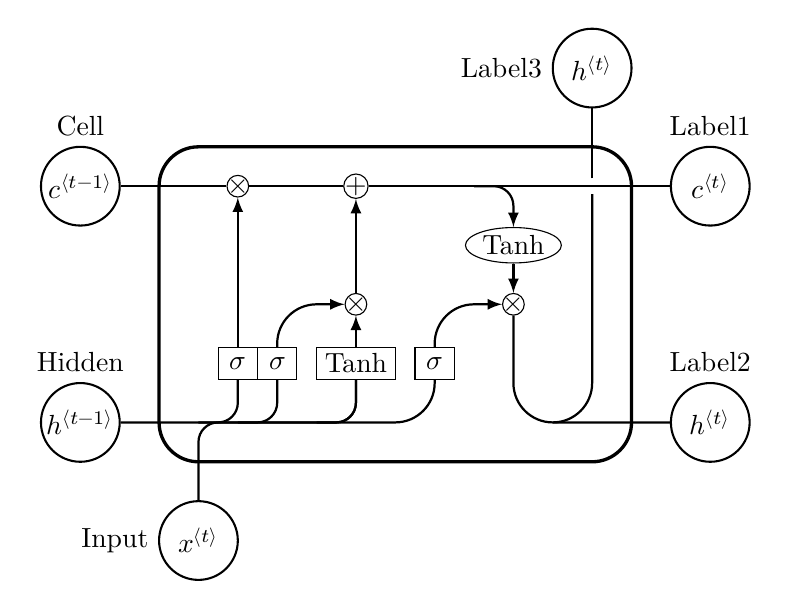
\begin{tikzpicture}[
    % GLOBAL CFG
    %font=\sf \scriptsize,
    %>=LaTeX,
    % Styles
    cell/.style={% For the main box
        rectangle, 
        rounded corners=5mm, 
        draw,
        very thick,
        },
    operator/.style={%For operators like +  and  x
        circle,
        draw,
        inner sep=-0.5pt,
        minimum height =.2cm,
        },
    function/.style={%For functions
        ellipse,
        draw,
        inner sep=1pt
        },
    gct/.style={% For external inputs and outputs
        circle,
        draw,
        line width = .75pt,
        minimum width=1cm,
        inner sep=1pt,
        },
    gt/.style={% For internal inputs
        rectangle,
        draw,
        minimum width=5mm,
        minimum height=4mm,
        inner sep=1pt
        },
    mylabel/.style={% something new that I have learned
        font=\scriptsize\sffamily
        },
    ArrowC1/.style={% Arrows with rounded corners
        rounded corners=.25cm,thick,
        },
    ArrowC2/.style={% Arrows with big rounded corners
        rounded corners=.5cm,
        thick,
        },
    ]

%Start drawing the thing...    
    % Draw the cell: 
    \node [cell, minimum height =4cm, minimum width=6cm] at (0,0){} ;

    % Draw inputs named ibox#
    \node [gt] (ibox1) at (-2,-0.75) {$\sigma$};
    \node [gt] (ibox2) at (-1.5,-0.75) {$\sigma$};
    \node [gt, minimum width=1cm] (ibox3) at (-0.5,-0.75) {Tanh};
    \node [gt] (ibox4) at (0.5,-0.75) {$\sigma$};

   % Draw opérators   named mux# , add# and func#
    \node [operator] (mux1) at (-2,1.5) {$\times$};
    \node [operator] (add1) at (-0.5,1.5) {+};
    \node [operator] (mux2) at (-0.5,0) {$\times$};
    \node [operator] (mux3) at (1.5,0) {$\times$};
    \node [function] (func1) at (1.5,0.75) {Tanh};

    % Draw External inputs? named as basis c,h,x
    \node[gct, label={Cell}] (c) at (-4,1.5) {\empt{c}{t-1}};
    \node[gct, label={Hidden}] (h) at (-4,-1.5) {\empt{h}{t-1}};
    \node[gct, label={left:Input}] (x) at (-2.5,-3) {\empt{x}{t}};

    % Draw External outputs? named as basis c2,h2,x2
    \node[gct, label={Label1}] (c2) at (4,1.5) {\empt{c}{t}};
    \node[gct, label={Label2}] (h2) at (4,-1.5) {\empt{h}{t}};
    \node[gct, label={left:Label3}] (x2) at (2.5,3) {\empt{h}{t}};

% Start connecting all.
    %Intersections and displacements are used. 
    % Drawing arrows    
    \draw [ArrowC1] (c) -- (mux1) -- (add1) -- (c2);

    % Inputs
    \draw [ArrowC2] (h) -| (ibox4);
    \draw [ArrowC1] (h -| ibox1)++(-0.5,0) -| (ibox1); 
    \draw [ArrowC1] (h -| ibox2)++(-0.5,0) -| (ibox2);
    \draw [ArrowC1] (h -| ibox3)++(-0.5,0) -| (ibox3);
    \draw [ArrowC1] (x) -- (x |- h)-| (ibox3);

    % Internal
    \draw [->, ArrowC2] (ibox1) -- (mux1);
    \draw [->, ArrowC2] (ibox2) |- (mux2);
    \draw [->, ArrowC2] (ibox3) -- (mux2);
    \draw [->, ArrowC2] (ibox4) |- (mux3);
    \draw [->, ArrowC2] (mux2) -- (add1);
    \draw [->, ArrowC1] (add1 -| func1)++(-0.5,0) -| (func1);
    \draw [->, ArrowC2] (func1) -- (mux3);

    %Outputs
    \draw [-, ArrowC2] (mux3) |- (h2);
    \draw (c2 -| x2) ++(0,-0.1) coordinate (i1);
    \draw [-, ArrowC2] (h2 -| x2)++(-0.5,0) -| (i1);
    \draw [-, ArrowC2] (i1)++(0,0.2) -- (x2);

\end{tikzpicture}
}

\end{figure}
\end{frame}

\end{document}
